\documentclass{classrep}
\usepackage[utf8]{inputenc}
\frenchspacing

\usepackage{graphicx}
\usepackage[usenames,dvipsnames]{color}
\usepackage[hidelinks]{hyperref}
\usepackage{lmodern}
\usepackage{graphicx}
\usepackage{placeins}
\usepackage{url}
\usepackage{amsmath, amssymb, mathtools}
\usepackage{listings}
\usepackage{fancyhdr, lastpage}

\pagestyle{fancyplain}
\fancyhf{}
\renewcommand{\headrulewidth}{0pt}
\cfoot{\thepage\ / \pageref*{LastPage}}

%--------------------------------------------------------------------------------------%
\studycycle{Informatyka, studia dzienne, inż I st.}
\coursesemester{VI}

\coursename{Sztuczna inteligencja i systemy ekspertowe}
\courseyear{2019/2020}

\courseteacher{dr inż. Krzysztof Lichy}
\coursegroup{wtorek, 12:15}

\author{%
    \studentinfo{Jan Karwowski}{216793}\\
    \studentinfo{Kamil Kowalewski}{216806}%
}

\title{Zadanie 1: Piętnastka}

\begin{document}
    \maketitle
    \thispagestyle{fancyplain}

    \section{Cel} {
        Celem zadania było stworzenie programu do rozwiązywania Piętnastki, czyli
        gry logicznej z wykorzystaniem różnych metod wyszukiwania rozwiązania
        i zbadanie ich skuteczności.
    }
%--------------------------------------------------------------------------------------%
    \section{Wprowadzenie} {
        Piętnastka to układanka posiadająca planszę 4 × 4 (16 miejsc) oraz 15 kwadratowych
        klocków o takich samych wymiarach, które są numerowane od 1 do 15 i są umieszczone
        na ww. planszy. Zawsze jedno miejsce pozostaje puste w celu zapewnienia możliwości przesuwania
        kloców, aby można było je ułożyć wg numerów w kolejności rosnącej. Możliwe są inne
        warianty tej gry - inny kształt planszy np. 4 × 3 lub inne jej wymiary np. 6 x 6, za czym
        idzie inna liczba klocków, aby wypełnić daną planszę i pozostawić jedno wolne miejsce.\\

        Szukanie rozwiązań jest to tak naprawdę przeszukiwanie drzewa. Wierzchołkami są aktualne
        ułożenia klocków tzn stany a pojedyńcze ruchy są krawędziami drzewa. Do odnalezienia
        ścieżki użyliśmy trzy strategie przeszukiwania drzewa:
        \begin{itemize}
            \item{DFS} - Przeszukiwanie w głąb
            \item{BFS} - Przeszukiwanie wszerz
            \item{A*} - Algorytm heurystyczny
        \end{itemize}

        \subsection{DFS - Przeszukiwanie w głąb} {
            Polega na przechodzeniu drzewa od zadanego wierzchołka (początkowy układ gry)
            do kolejnych jego potomków i jest to powtarzane dla każdego kolejnego potomka. Gdy
            dany węzeł nie ma już potomka algorytm wraca o jeden poziom i przechodzi do innych
            węzłów, które nie zostały jeszcze sprawdzone. Mówiąc obrazowo algorytm przechodzi po
            węzłach aż do samego dołu drzewa (idzie pionowo) i jeśli nie, znajdzie rozwiązania to
            wraca do góry i sprawdza kolejne aż do znalezienia rozwiązania.
        }

        \subsection{BFS - Przeszukiwanie wszerz} {
            Polega na przechodzeniu drzewa od zadanego wierzchołka (początkowy układ gry)
            do kolejnego węzła poziomami na tym samym poziomie. Jeżeli na danym poziomo
            zostaną sprawdzone wszystkie węzły nie zostanie znalezione rozwiązanie algorytm
            przechodzi jeden poziom niżej i kontynuuje sprawdzanie.
        }

        \subsection{A* - Algorytm heurystyczny} {
            Polega na przeszukiwaniu w pierwszej kolejności węzłów, dla których wartość funkcji
            f(x) jest najmniejsza:
            \begin{align*}
                f(x)=g(x)+h(x)
            \end{align*}
            gdzie:\\
            g(x) to funkcja kosztu(zwraca jak głeboko jest stan)\\
            h(x) to funkcja heurystyczna\\

            Zostały wykorzystane dwie metryki:
            \begin{itemize}
                \item{Hamminga} - obliczane jest ile klocków nie znajduję się na właściwym miejscu
                \item{Manhattan} - obliczane jest ile ruchów jest potrzebne do osiągniecia
                docelowych miejsc(kolumny+wiersze)
            \end{itemize}
        }
    }
%--------------------------------------------------------------------------------------%
    \section{Opis implementacji} {
        Program został stworzony jako aplikacja konsolowa w języku C. Potrzebne parametry
        do działania programu przekazywane np. rodzaj algorytmu, priorytet ruchów,
        plik zawierający początkowy stanem układanki są przekazywane jako parametry wywołania
        programu.

        Podstawowym obiektem reprezentującym pojedynczy stan gry oraz jednokierunkową listę kroków
        potrzebnych, aby ten stan osiągnąć, jest struktura 'GameState'. Zostały zaimplementowane
        dwie podstawowe operacje, które na tej strukturze można wykonać:
        \begin{itemize}
            \item step - jeżeli możliwe wykonuje ruch pustym polem w zadanym
            kierunku, w przeciwnym wypadku zwraca 0
            \item back - jeżeli możliwe cofa poprzedni ruch (wykonuje ruch w przeciwną stronę
            do ostatniego), w przypadku gdy wszystkie ruchy zostały cofnięte zwraca 0
        \end{itemize}
        Ponadto stworzone zostały funkcje pomocnicze służące do inicjalizacji, zwolnienia
        pamięci i tworzenia kopii stanu oraz funkcja pozwalająca stwierdzić, czy dany
        stan jest już rozwiązaniem gry.

        Wspomniane dwie podstawowe operacje są w pewnym uproszczeniu wykonywane 'in situ'
        (bez uwzględnienia dynamicznej listy kroków, która będzie rosnąć proporcjonalnie do
        długości rozwiązania). Ze względu na fakt, że wszystkie możliwe do utworzenia stany są
        jednoznacznie identyfikowane i możliwe do odtworzenia na podstawie stanu początkowego i
        listy kroków, oraz dlatego, że algorytm generowania kolejnych stanów jest bardzo mało
        skomplikowany, zdecydowaliśmy się w tej konkretnej implementacji, przetrzymywać w pamięci
        tylko jeden stan i modyfikować go wykorzystując dwie bazowe operacje - 'step' i 'back'.


        \subsection{DFS} {
            Algorytm przeszukiwania w głąb został zaimplementowany rekurencyjnie. Maksymalna
            głębokość rekurencji została na stałe ustawiona na 20. Algorytm aż do osiągnięcia
            zadanej głębokości będzie dokonywał kolejnych wywołań rekurencyjnych na węzłach
            potomnych (tworzonych dynamicznie). Przy przechodzeniu do węzła potomnego wykorzystywana
            jest operacja 'step', natomiast podczas wychodzenia z kolejnych rekurencji wykorzystywana
            jest operacja 'back'. Węzeł stanu jest uznany za odwiedzony, kiedy została na nim
            wywołana rekurencyjna funkcja 'DFS'. Jeżeli doszło do próby zagnieżdżenia się w
            węzły potomne taki stan uznany jest także za przetworzony.
        }

        \subsection{BFS} {
            Algorytm przeszukiwania wszerz został zaimplementowany iteracyjnie. Algorytm sprowadza
            się do utworzenia listy reprezentującej wykonane kroki, potrzebne do osiągnięcia
            rozpatrywanego węzła stanu gry. W kolejnych iteracjach ostatni krok tej listy jest
            zmieniany na kolejny (co wynika z zadanej kolejności badania kroków, np. LURD),
            wykonywana jest więc za każdym razem operacja najpierw 'back', a później 'next' z
            nowym parametrem. Jeżeli wszystkie cztery stany zostały przebadane następuje
            "zawinięcie" i krok poprzedni zostaje zmieniony na kolejny. Kiedy tą metodą
            sprawdzone zostaną wszystkie wariacje z powtórzeniami dla danej liczby kroków,
            liczba kroków zostaje zwiększona i cała operacja powtarza się w sposób analogiczny.
            Ze względu na specyficzną, wynikającą z wyobraźni autora implementację algorytmu,
            nie zostały w żaden sposób rozróżnione węzły odwiedzone i przetworzone.
        }

        \subsection{A*} {
            Algorytm A-star został zaimplementowany również przy wykorzystaniu dwóch podstawowych
            operacji: 'back' i 'step'. Metoda ta polega na wybieraniu w każdym kolejnym kroku,
            ze wszystkich (2, 3 lub 4 możliwości) tej, która spowoduje powstanie stanu
            bliższego - bardziej podobnego (według pewnej metryki) stanowi końcowemu - rozwiązaniu.
            Wykorzystano dwie metryki - metryka Hamminga i metryka Manhattan. Aby algorytm ten
            działał poprawnie wymagane jest w każdym kolejnym kroku sprawdzanie, czy powstały stan
            nie został przebadany już wcześniej, w przeciwnym przypadku dojdzie to zapętlenia
            algorytmu. Jeżeli nie jest możliwe wykonanie żadnego kroku, który generowałby nowy
            stan, oznacza to, że algorytm nie jest w stanie rozwiązać zadania. Sprawdzenie czy
            węzeł stanu był już wcześniej sprawdzony dokonywane jest poprzez utworzenie pojedynczej
            kopii stanu głównego i wielokrotne wykonanie operacji 'back'. Podobnie jak w przypadku
            algorytmu BFS nie zostało uwzględnione rozróżnienie między stanami odwiedzonymi
            a przetworzonymi - istnieje bowiem tylko i wyłącznie jeden stan, który cały
            czas jest modyfikowany.
        }
    }
%--------------------------------------------------------------------------------------%
    \section{Materiały i metody} {
        Do badań zostały użyte skrypty i programy dostępne na stronie przedmiotów do
        generowania danych. Dzięki nim zostały stworzone wszystkie możliwe stany
        układanki o liczbie ruchów od 1 do 7.\\
        Dla algorytmów DFS i BFS zostały użyte następujące porządki przeszukiwania sąsiedztwa:
        \begin{itemize}
            \item prawo-dół-góra-lewo
            \item prawo-dół-lewo-góra
            \item dół-prawo-góra-lewo
            \item dół-prawo-lewo-góra
            \item lewo-góra-dół-prawo
            \item lewo-góra-prawo-dół
            \item góra-lewo-dół-prawo
            \item góra-lewo-prawo-dół
        \end{itemize}
        \bigskip

        Następnie nasz program został uruchomiony a wszystkie dane zostały odpowiednio pogrupowane
        (za pomocą skryptu edytora 'vim') i wykorzystane do wygenerowania wykresów z użyciem
        programu 'gnuplot'.
    }
%--------------------------------------------------------------------------------------%
    \section{Wyniki} {
        Zostały przebadane 413 układów.
        Algorytmy typu 'brute-force', czyli DFS i BFS za każdym razem znalazły poprawne rozwiązanie
        zadania. Algorytmy heurystyczne, co wynika z ich natury, w niektórych przypadkach nie
        znalazły poprawnego rozwiązania. Liczba błędów popełnionych przez algorytmy heurystyczne
        przedstawia się następująco:
        \begin{figure}[!htbp]
            \centering
            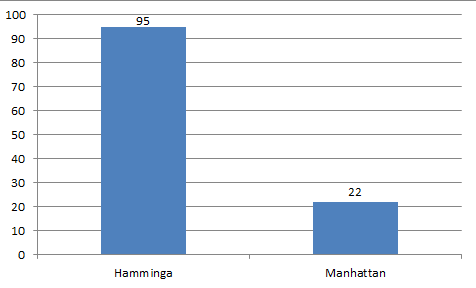
\includegraphics[width=\textwidth, width=90mm]{img/NumberOfErrors.png}
            \caption{Liczba pomyłek}
            \label{NumberOfErrors}
        \end{figure}


        Poniżej, na podstawie przeprowadzonych doświadczeń, w sposób graficzny przedstawione
        zostały średnie wartości następujących parametrów dla każdego algorytmu z osobna i zbiorczo,
        dla wszystkich algorytmów razem, aby umożliwić ich łatwiejsze porównanie.
        \begin{itemize}
            \item średnia długość znalezionego rozwiązania
            \item średnia liczba stanów odwiedzonych
            \item średnia maksymalna osiągnięta głębokość rekursji
            \item średni czas trwania procesu obliczeniowego
        \end{itemize}
        Ze względu na wynikający z implementacji bądź głupoty autorów brak znaczenia parametru
        liczby stanów przetworzonych, wartość ta nie zostaje uwzględniona w przedstawionych podsumowaniach.

%        \begin{figure}[!htbp]
%            \centering
%            \includegraphics[width=\textwidth, width=80mm]{img/.png}
%            \caption{Podpis pod rysunkiem}
%        \end{figure}

        \subsection{BFS}{
            \begin{figure}[!htbp]
                \centering
                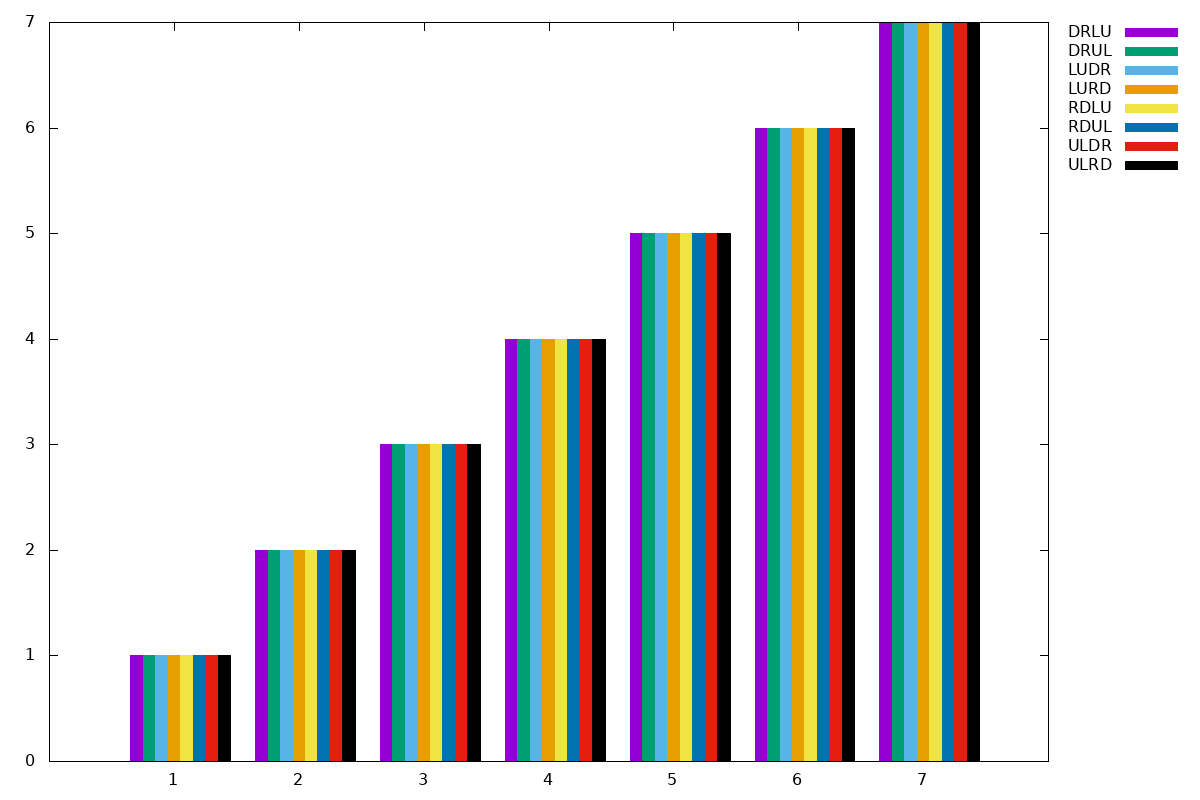
\includegraphics[width=\textwidth, height=55mm]{img/BFS_depth.png}
                \caption{X - liczba kroków rozwiązania, Y - średnia głębokość rekursji}
                \label{BFS_depth}
            \end{figure}

            \begin{figure}[!htbp]
                \centering
                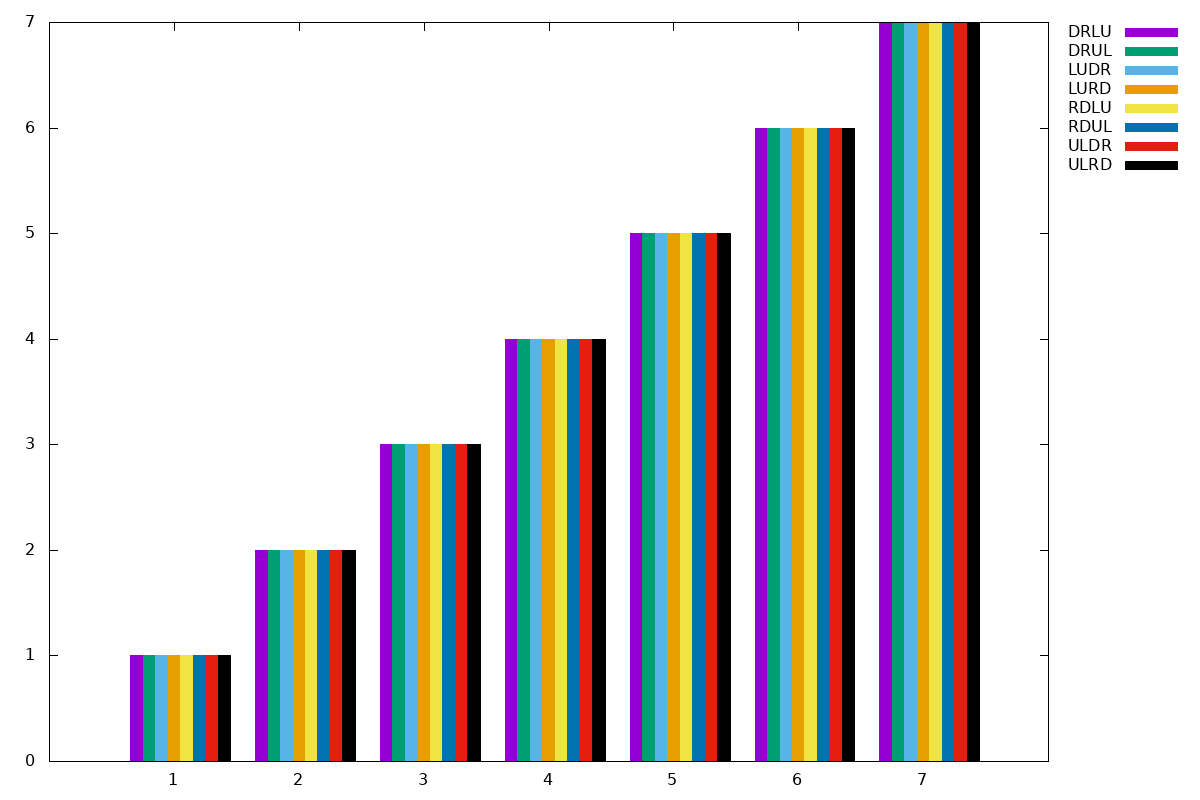
\includegraphics[width=\textwidth, height=55mm]{img/BFS_length.png}
                \caption{X - liczba kroków rozwiązania, Y - średnia długość rozwiązania}
                \label{BFS_length}
            \end{figure}

            \begin{figure}[!htbp]
                \centering
                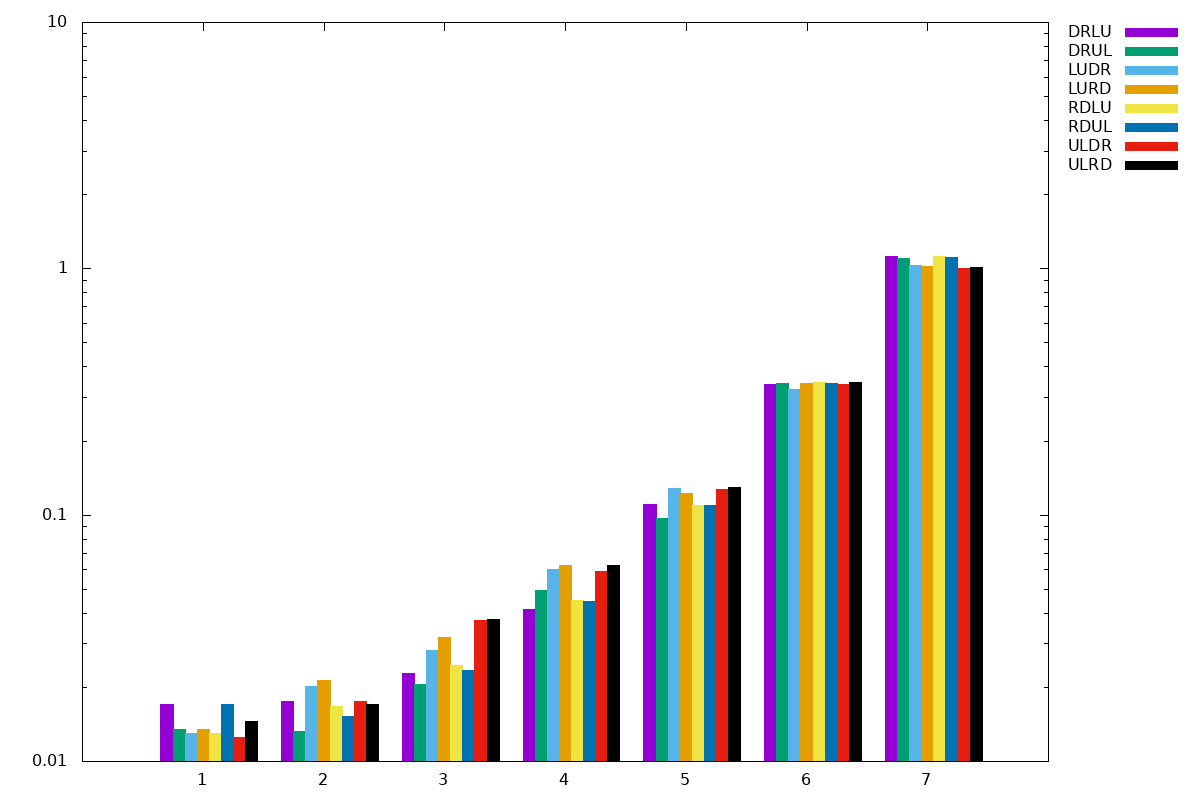
\includegraphics[width=\textwidth, height=55mm]{img/BFS_time.png}
                \caption{X - liczba kroków rozwiązania, Y - średni czas potrzebny na rozwiązanie}
                \label{BFS_time}
            \end{figure}

            \begin{figure}[!htbp]
                \centering
                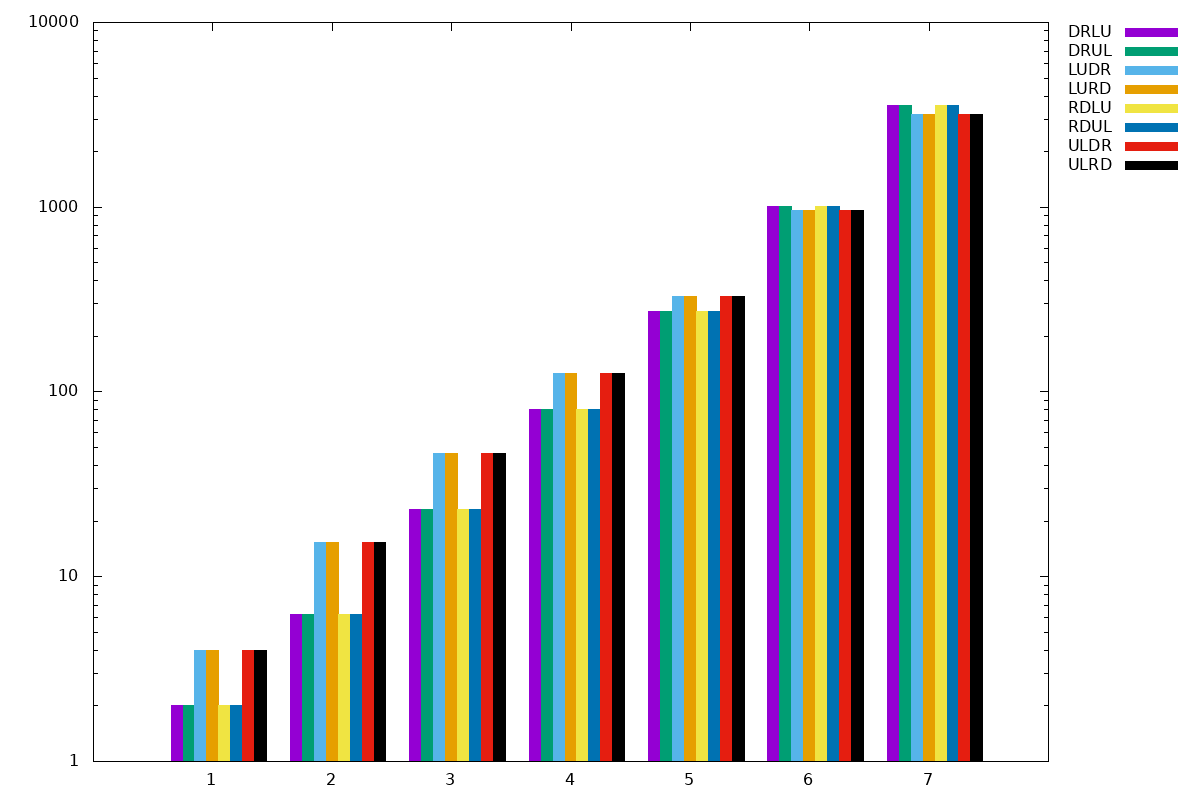
\includegraphics[width=\textwidth, height=55mm]{img/BFS_visited.png}
                \caption{X - liczba kroków rozwiązania, Y - średnia liczba odwiedzonych węzłów}
                \label{BFS_visited}
            \end{figure}
            \FloatBarrier
        }

        \subsection{DFS} {
            \begin{figure}[!htbp]
                \centering
                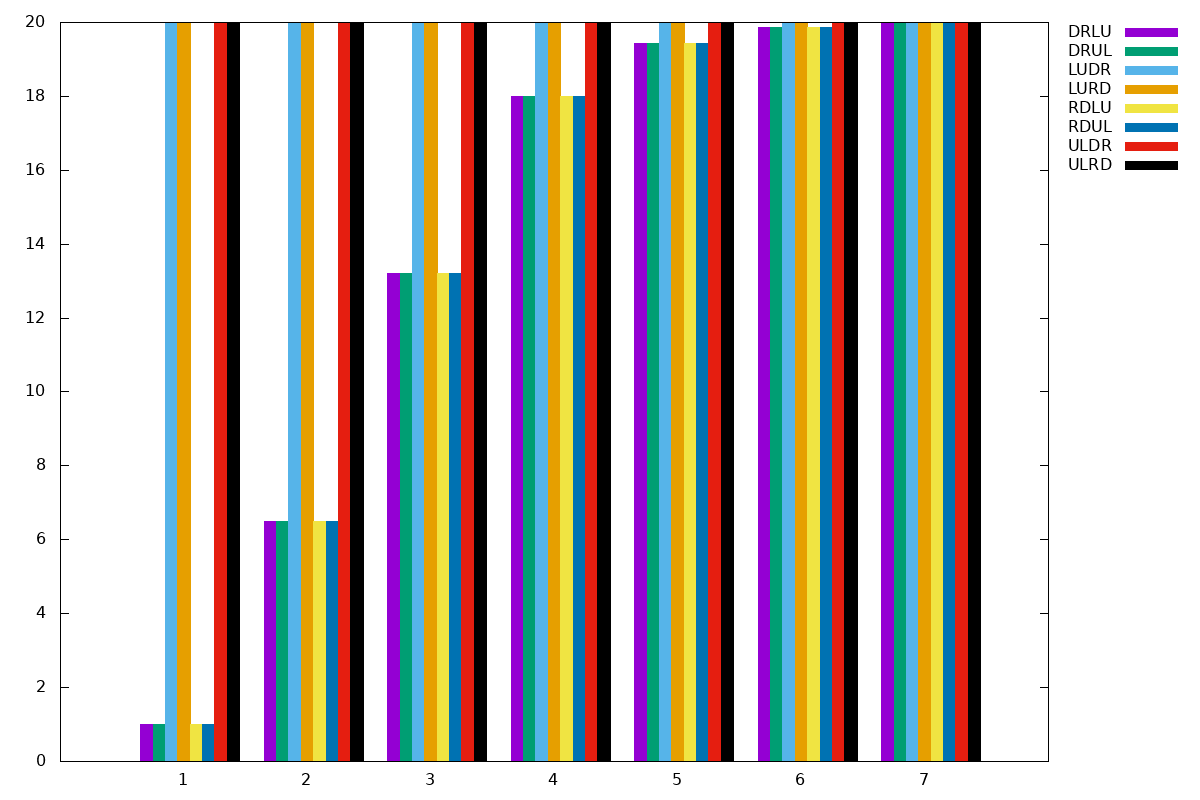
\includegraphics[width=\textwidth, height=55mm]{img/DFS_depth.png}
                \caption{X - liczba kroków rozwiązania, Y - średnia głębokość rekursji}
                \label{DFS_depth}
            \end{figure}

            \begin{figure}[!htbp]
                \centering
                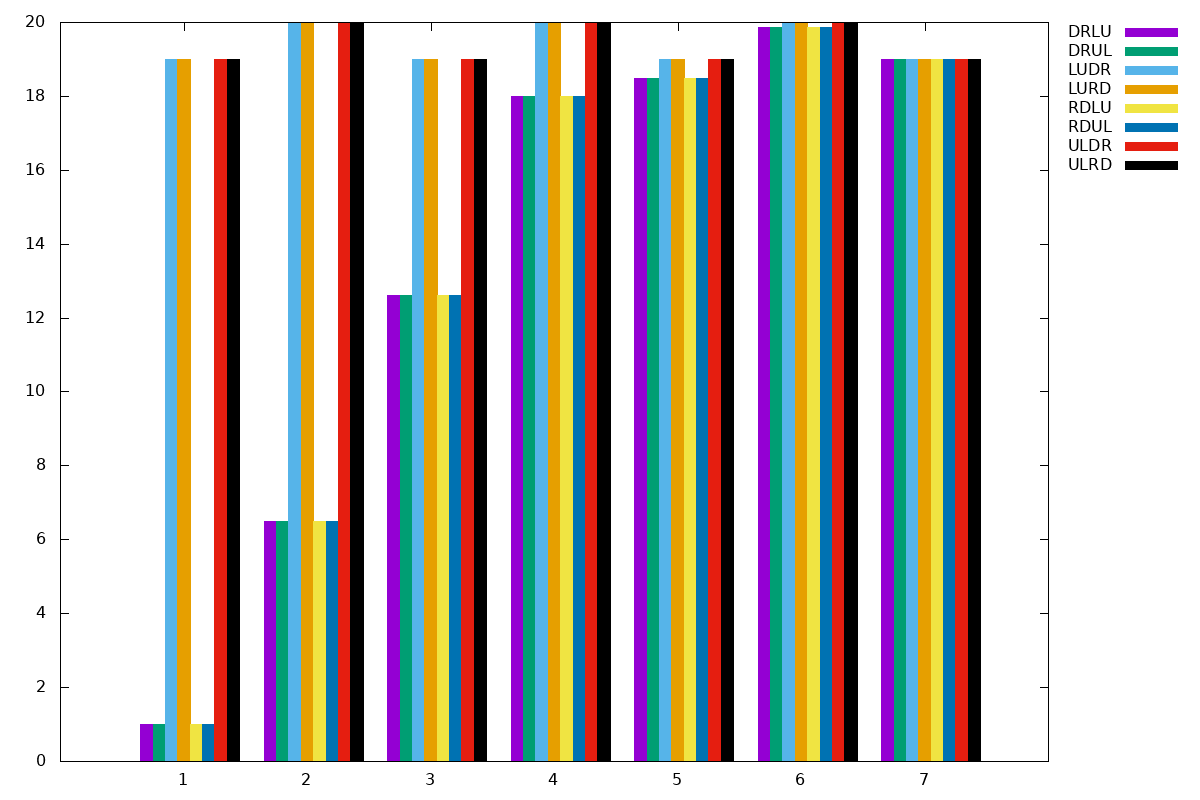
\includegraphics[width=\textwidth, height=55mm]{img/DFS_length.png}
                \caption{X - liczba kroków rozwiązania, Y - średnia długość rozwiązania}
                \label{DFS_length}
            \end{figure}

            \begin{figure}[!htbp]
                \centering
                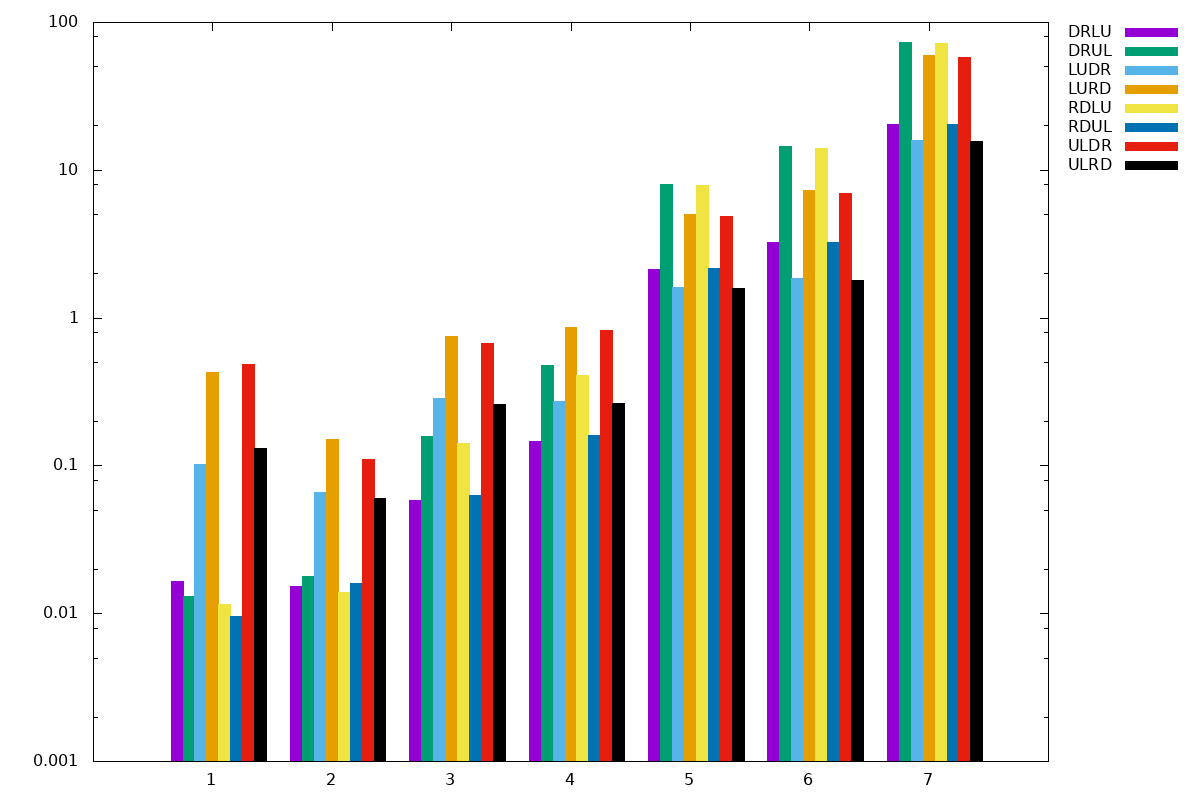
\includegraphics[width=\textwidth, height=55mm]{img/DFS_time.png}
                \caption{X - liczba kroków rozwiązania, Y - średni czas potrzebny na rozwiązanie}
                \label{DFS_time}
            \end{figure}

            \begin{figure}[!htbp]
                \centering
                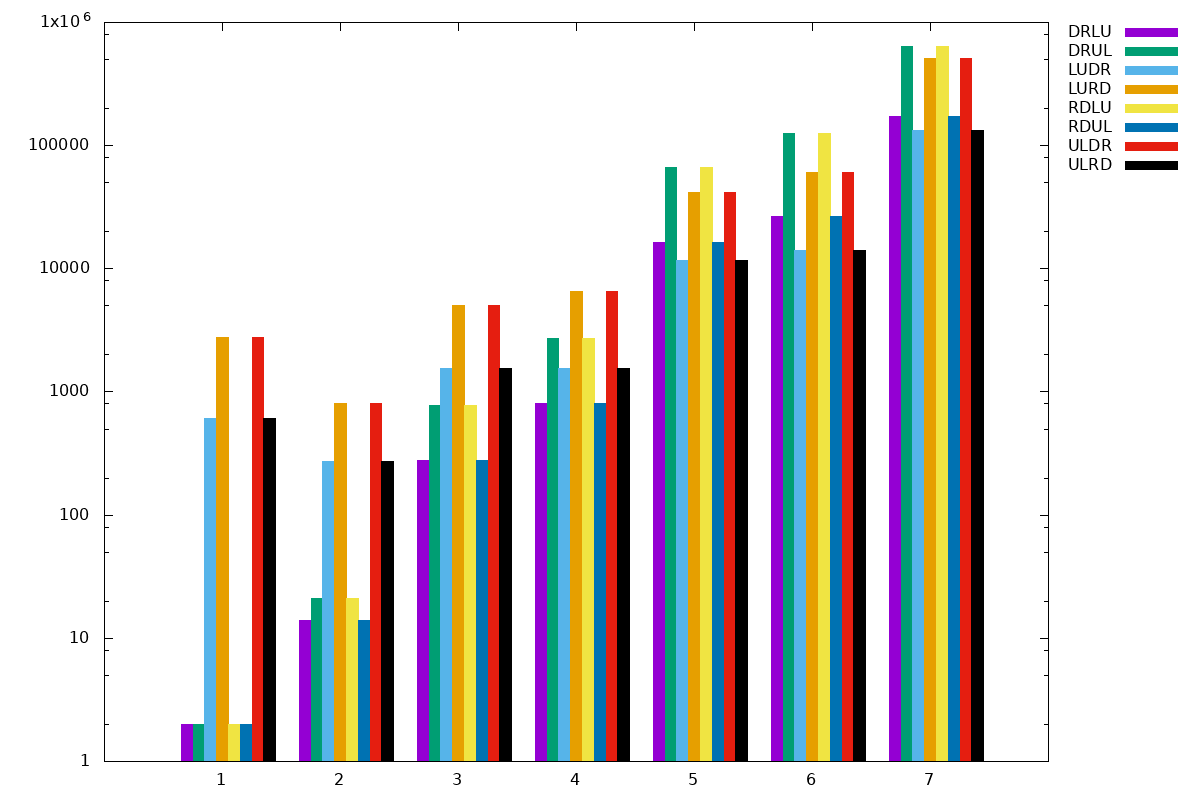
\includegraphics[width=\textwidth, height=55mm]{img/DFS_visited.png}
                \caption{X - liczba kroków rozwiązania, Y - średnia liczba odwiedzonych węzłów}
                \label{DFS_visited}
            \end{figure}
            \FloatBarrier
        }

        \subsection{A*} {
            \begin{figure}[!htbp]
                \centering
                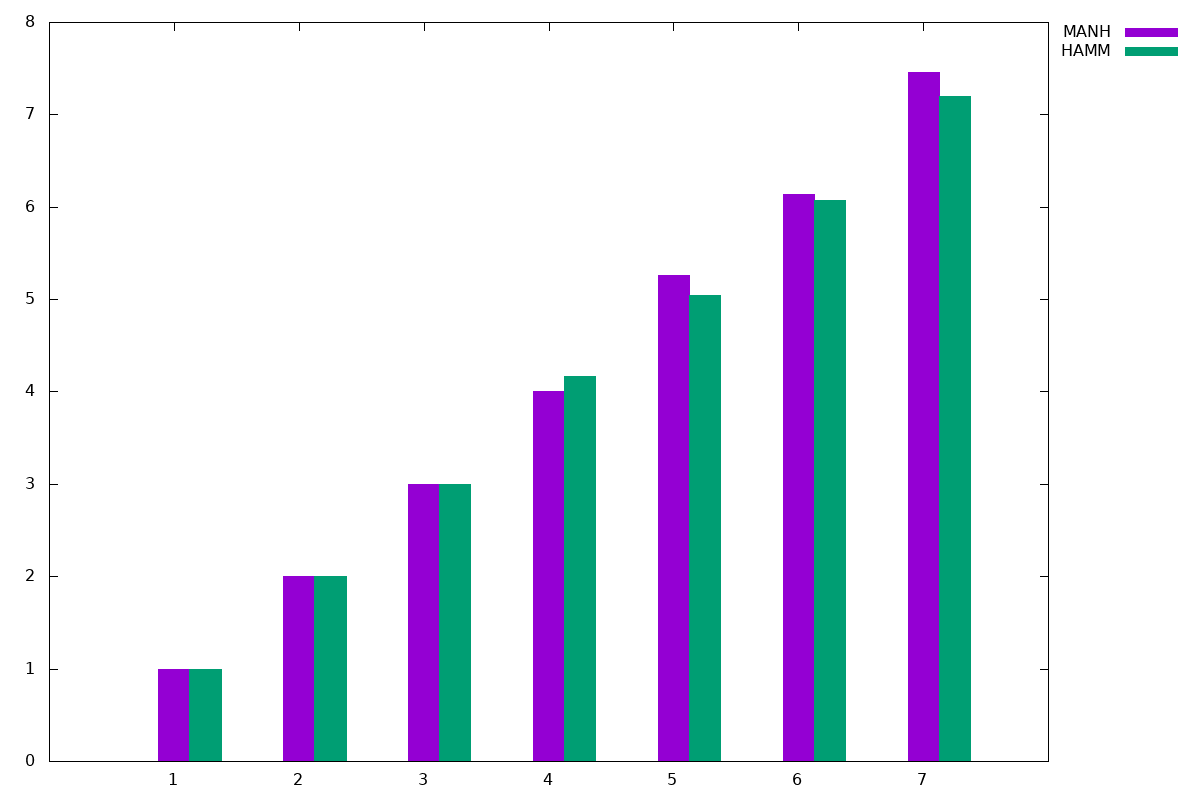
\includegraphics[width=\textwidth, height=55mm]{img/ASTR_depth.png}
                \caption{X - liczba kroków rozwiązania, Y - średnia głębokość rekursji}
                \label{ASTR_depth}
            \end{figure}

            \begin{figure}[!htbp]
                \centering
                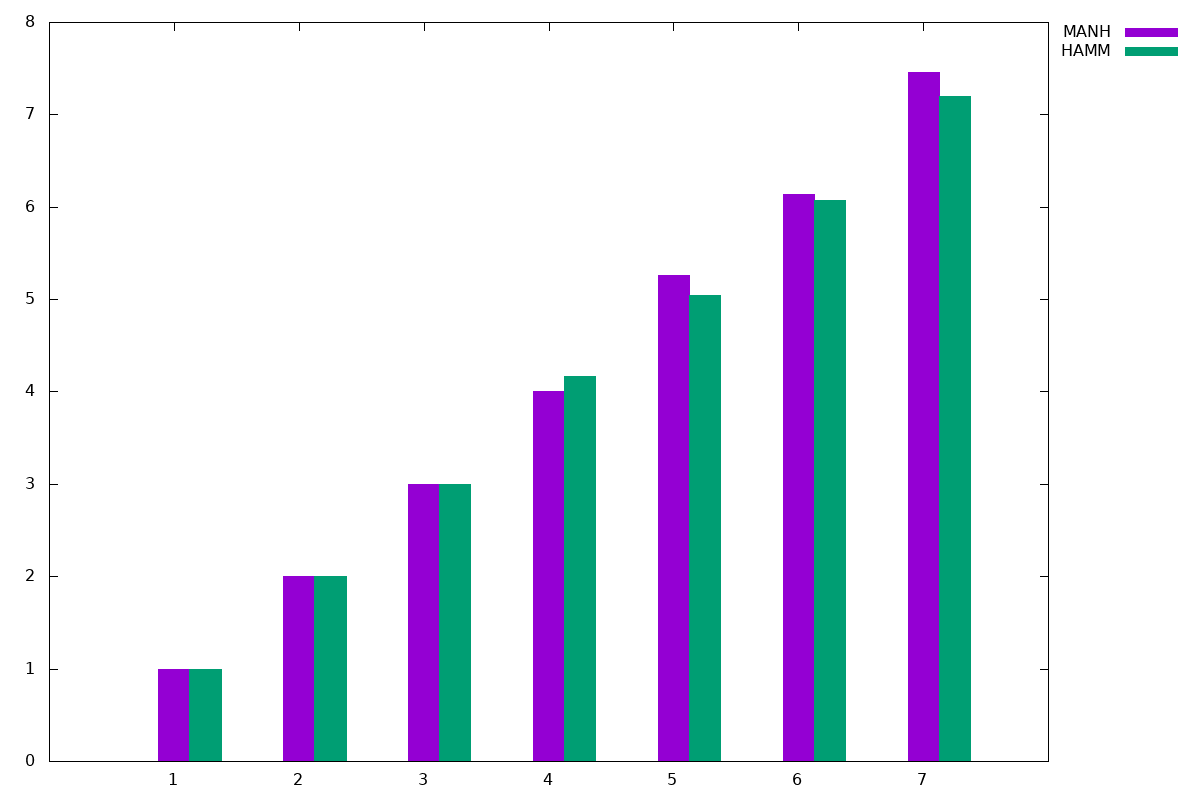
\includegraphics[width=\textwidth, height=55mm]{img/ASTR_length.png}
                \caption{X - liczba kroków rozwiązania, Y - średnia długość rozwiązania}
                \label{ASTR_length}
            \end{figure}

            \begin{figure}[!htbp]
                \centering
                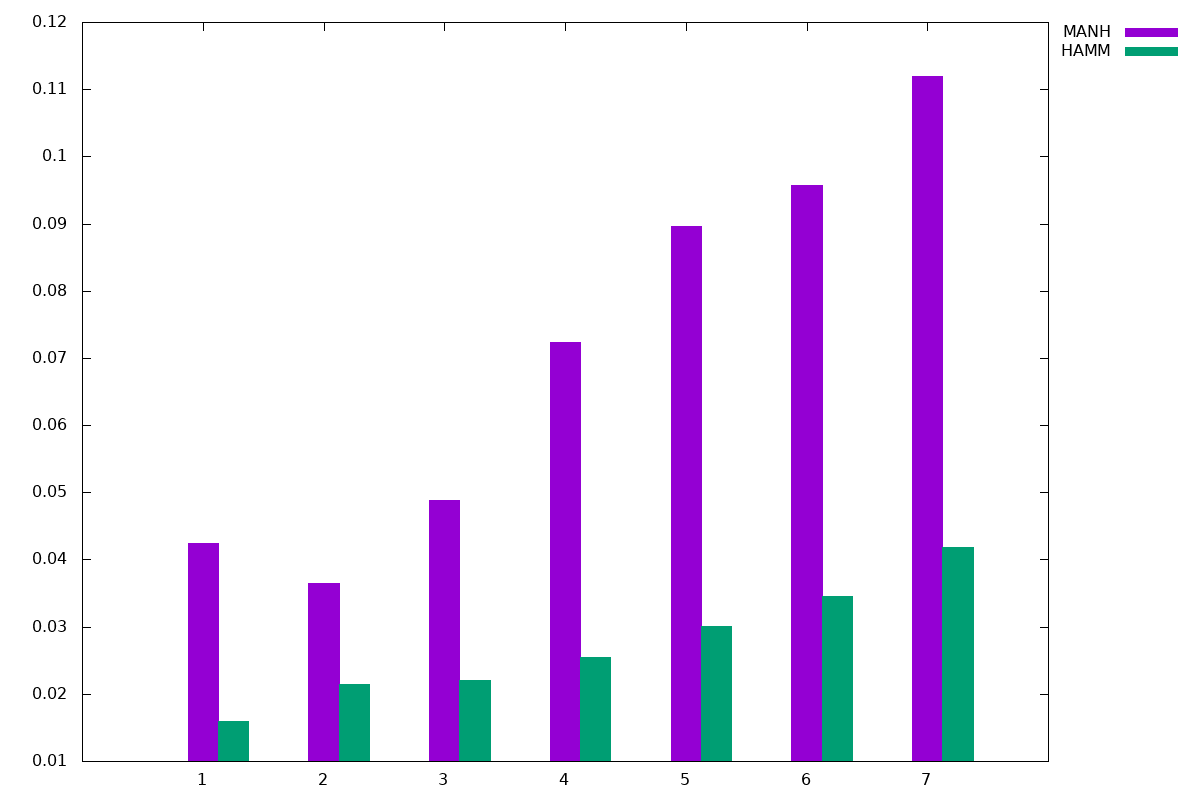
\includegraphics[width=\textwidth, height=55mm]{img/ASTR_time.png}
                \caption{X - liczba kroków rozwiązania, Y - średni czas potrzebny na rozwiązanie}
                \label{ASTR_time}
            \end{figure}

            \begin{figure}[!htbp]
                \centering
                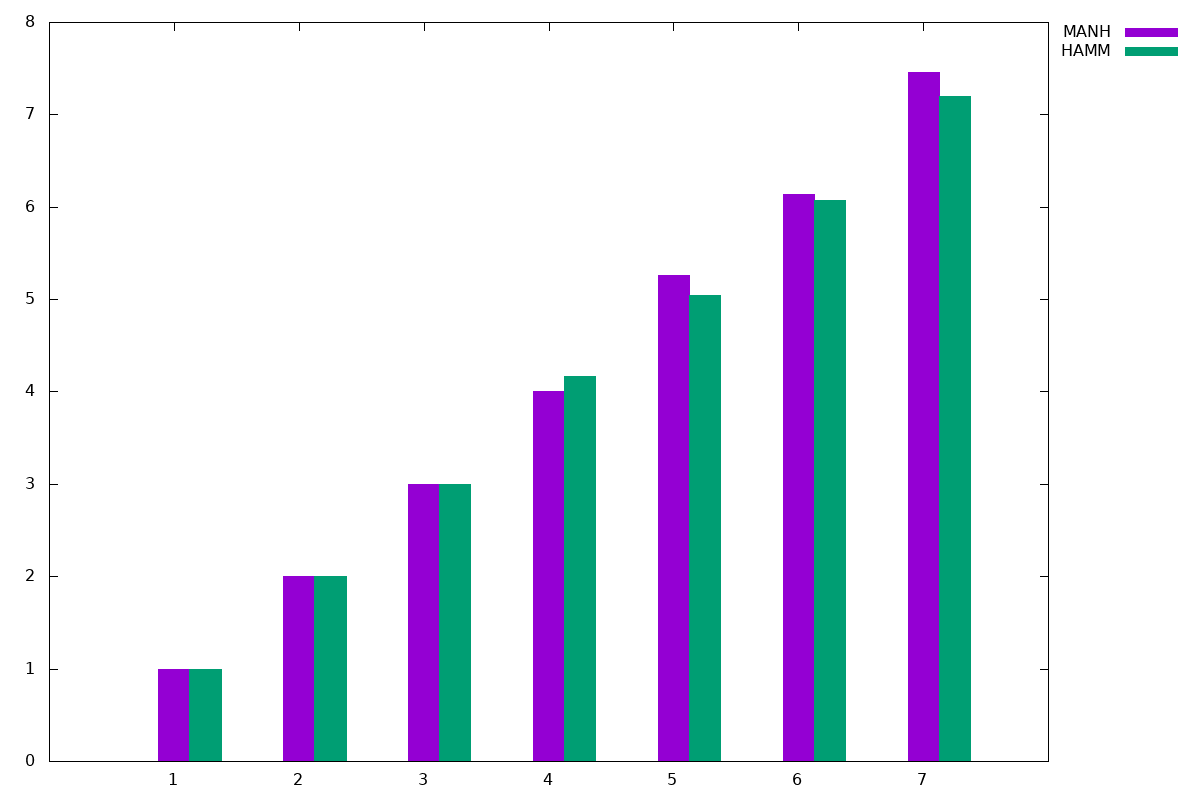
\includegraphics[width=\textwidth, height=55mm]{img/ASTR_visited.png}
                \caption{X - liczba kroków rozwiązania, Y - średnia liczba odwiedzonych węzłów}
                \label{ASTR_visited}
            \end{figure}
            \FloatBarrier
        }

        \subsection{Porównanie wszystkiech algorytmów} {
            \begin{figure}[!htbp]
                \centering
                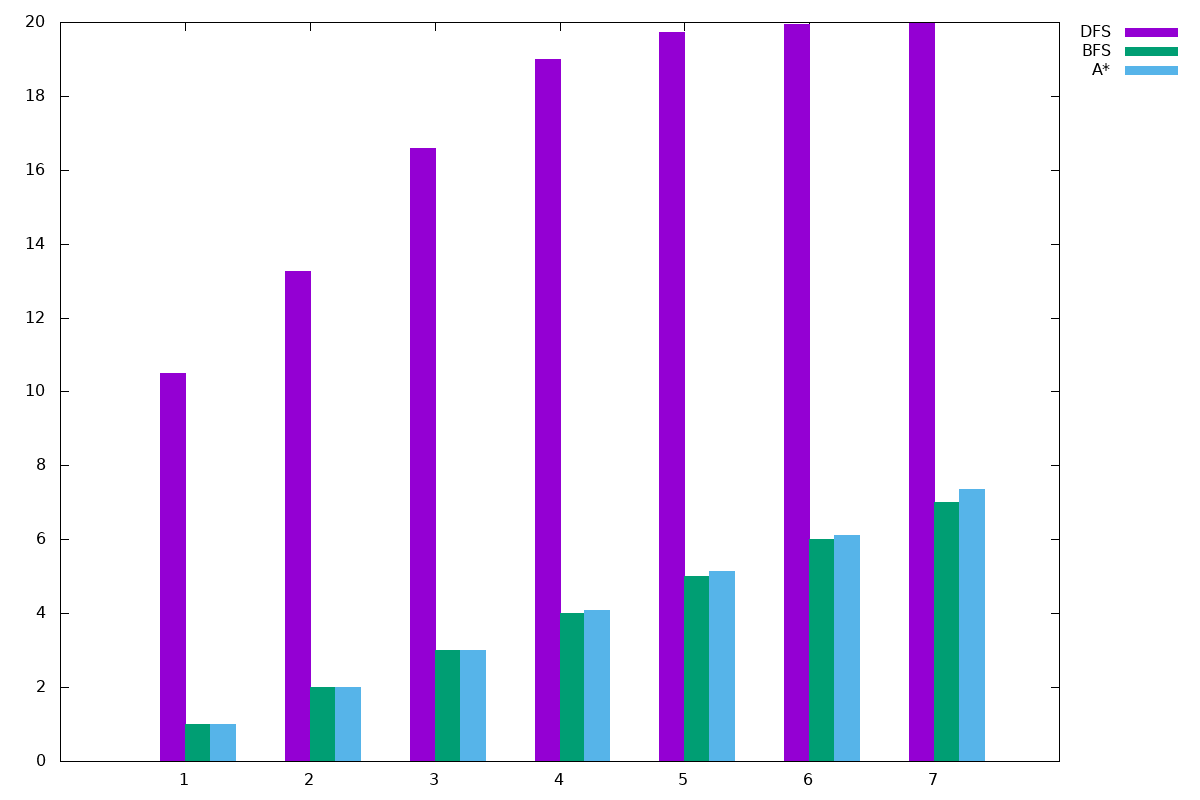
\includegraphics[width=\textwidth, height=55mm]{img/CMN_depth.png}
                \caption{X - liczba kroków rozwiązania, Y - średnia głębokość rekursji}
                \label{CMN_depth}
            \end{figure}

            \begin{figure}[!htbp]
                \centering
                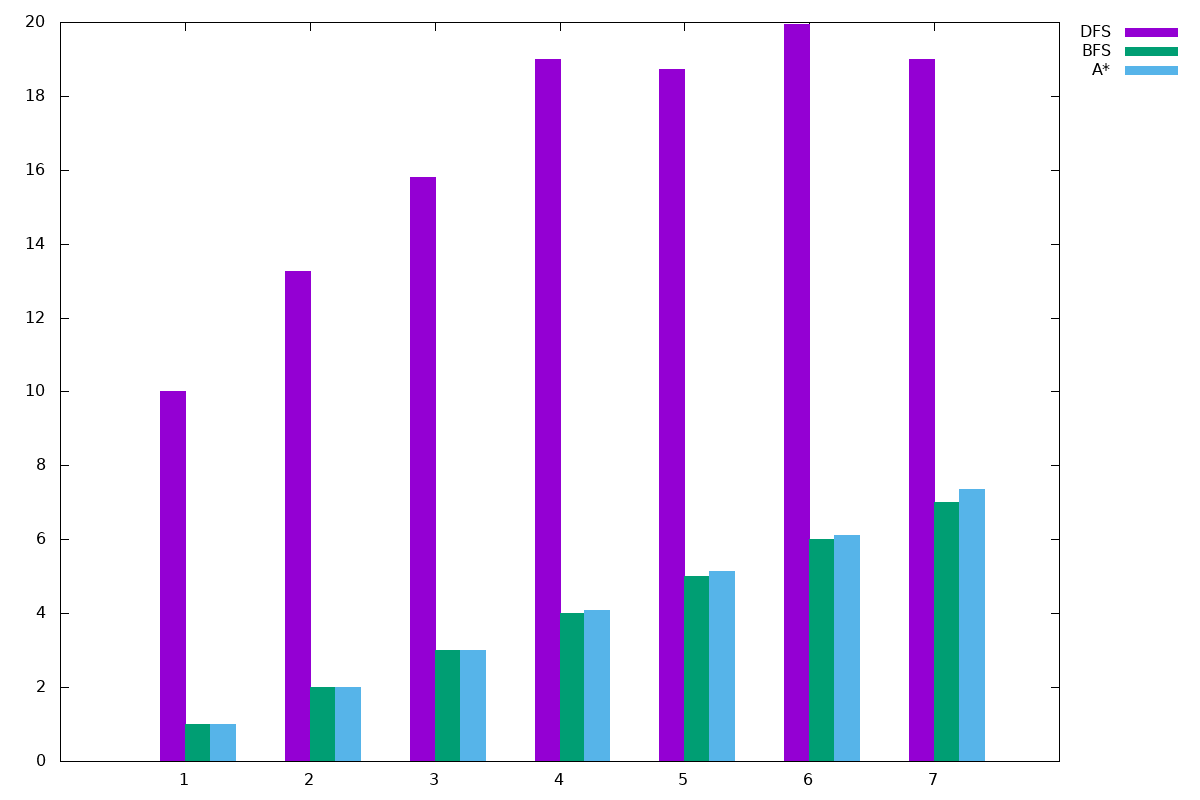
\includegraphics[width=\textwidth, height=55mm]{img/CMN_length.png}
                \caption{X - liczba kroków rozwiązania, Y - średnia długość rozwiązania}
                \label{CMN_length}
            \end{figure}

            \begin{figure}[!htbp]
                \centering
                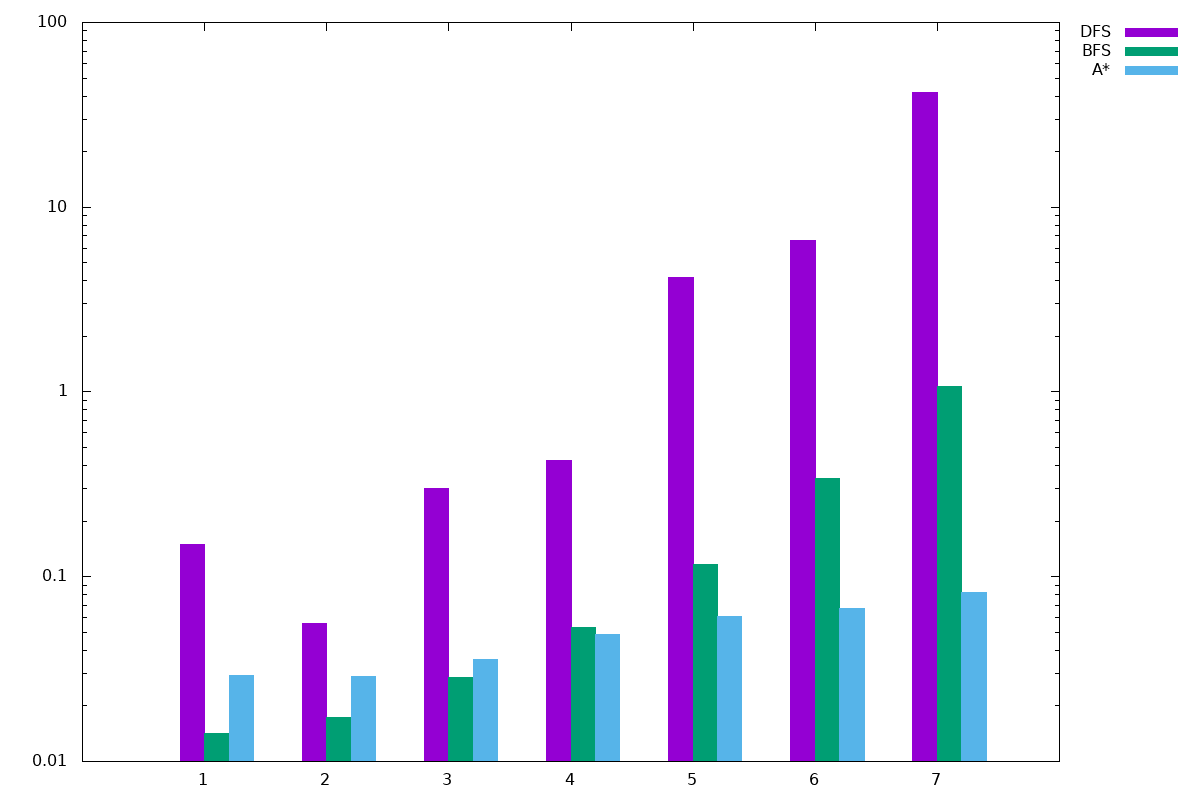
\includegraphics[width=\textwidth, height=55mm]{img/CMN_time.png}
                \caption{X - liczba kroków rozwiązania, Y - średni czas potrzebny na rozwiązanie}
                \label{CMN_time}
            \end{figure}

            \begin{figure}[!htbp]
                \centering
                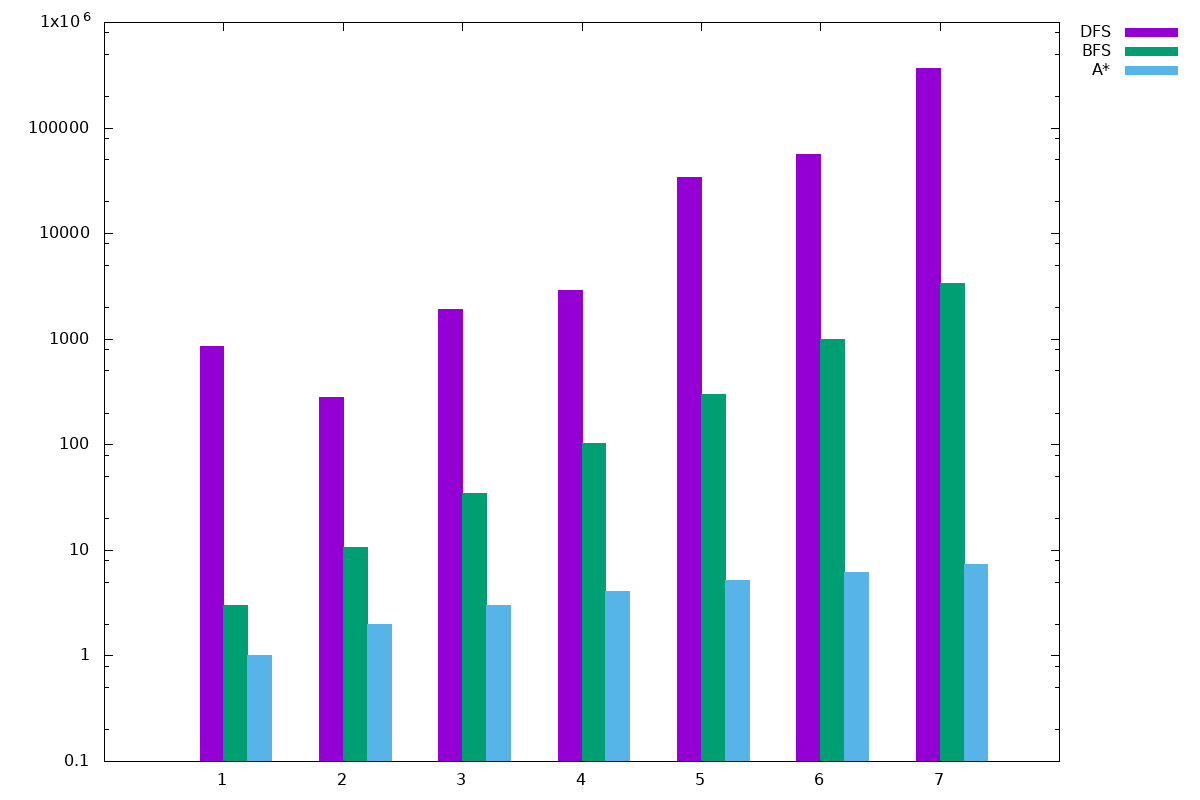
\includegraphics[width=\textwidth, height=55mm]{img/CMN_visited.png}
                \caption{X - liczba kroków rozwiązania, Y - średnia liczba odwiedzonych węzłów}
                \label{CMN_visited}
            \end{figure}
            \FloatBarrier
        }
    }
%--------------------------------------------------------------------------------------%
    \section{Dyskusja} {

        \subsection{DFS} {
            Algorytm przeszukiwania w głąb, jako że wszystkie rozpatrywane stany były
            zmodyfikowane o 7 lub mniej kroków od stanu początkowego, dla każdego przypadku
            znalazł poprawne rozwiązanie. Długość tego rozwiązania, co wynika z wykresu
            |\ref{DFS_depth}|, często nie jest równa faktycznej minimalnej liczbie kroków potrzebnych, aby otrzymać
            rozwiązanie gry. Wynika to z faktu, że algorytm praktycznie na samym początku schodzi
            do maksymalnej możliwej głębokości rekursji, a spośród stanów tam znalezionych,
            także może wyłonić ten, będący rozwiązaniem. Najbliższe rozwiązanie nie jest w tym
            przypadku rozwiązaniem najkrótszym. Warto zauważyć, że w zależności od wybranej
            kolejności kierunków kroków, algorytm ma dla różnych eksperymentów inne szanszę
            znaleźć rozwiązanie wcześniej bądź później. Jest to jednak kwestia losowa, co pozostaje
            zjawiskiem niekorzystnym, ponieważ istnieje możliwość wystąpienia scenariusza
            pesymistycznego, który będzie setki razy dłuższy niż scenariusz optymistyczny.
            Jest to widoczne na wykresie |\ref{DFS_time}|.


            Długość rozwiązania w przypadku tego algorytmu może być mniejsza niż maksymalna
            głębokość rekursji, co także wynika z faktu, że metoda DFS od samego początku
            schodzi na najniższy poziom. Liczba odwiedzonych stanów zachowuje się podobnie
            jak czas trwania pracy algorytmu. To znaczy rośnie wykładniczo wraz ze wzrostem
            liczby kroków rozwiązania i może się w przypadkach pesymistycznych róznić wiele
            rzędów wielkości od przypadków optymistycznych.
        }

        \subsection{BFS} {
            Długość znalezionego rozwiązania, jak i maksymalny poziom rekursji, w przypadku tego
            algorytmu zawsze będą wynosiły minimalną liczbę kroków rozwiązania minimalnego. Jest
            to widoczne na wykresach |\ref{BFS_depth}| i |\ref{BFS_length}|. Zachowanie to różni się znacznie
            od zachowania algorytmu DFS i wynika z kolejności przeszukiwania węzłów stanów. Jeżeli,
            tak jak się to właśnie w metodzie BFS odbywa, stany są przeszukiwane wszystkie na danym
            poziomie, to zawsze zostanie znalezione rozwiązanie najkrótsze. Zachowanie to jest
            bardzo pożądane, ponieważ nie dopuszcza przypadków pesymistycznych wynikających jedynie
            ze źle dobranej kolejności kierunków kroków, która w przypadku tego algorytmu nie
            wpływa znacząco na rozwiązanie.
            Liczba odwiedzonych stanów i czas trwania pracy algorytmu tutaj również rośnie
            wykładniczo wraz z dodawaniem kolejnych kroków do długości rozwiązania. Nie ma
            jednak, jak już wspomniano, tak widocznej różnicy dla różnych kolejności kierunków kroków.
        }

        \subsection{A*} {
            Metoda A-star różni się znacznie od dwóch poprzednich, gdyż po pierwsze, nie zawsze
            potrafi znaleźć poprawne rozwiązanie, po drugie wykonuje prawie że, tylko tyle kroków,
            ile potrzeba aby zadanie rozwiązać. Trzy wykresy |\ref{ASTR_depth}|, |\ref{ASTR_length}| i |\ref{ASTR_visited}|
            rosną liniowo, są właściwie dokładnie takie same i pokazują, że liczba odwiedzonych stanów,
            podobnie jak osiągnięta głębokość rekursji, jest równa zawsze długości rozwiązania
            (każdy odwiedzony stan jest dokładany do rozwiązania i interpretowany jako kolejny
            stopień rekurencji). Czas trwania pracy tego algorytmu rośnie zaledwie liniowo, jest
            proporcjonalny liczbie kroków rozwiązania. Wszystkie te parametry jednoznacznie wskazują
            na znaczną przewagę, w kategorii szybkości i ilości wykorzystanych zasobów,
            nad metodami BFS i DFS.

            Warto zwrócić uwagę, że dwie wykorzystane heurystyki zachowują się w sposób bardzo
            odmienny. Po pierwsze heurystyka Hamminga jest znacznie szybsza, co wynika z faktu,
            że obliczanie odległości z wykorzystaniem metryki Hamminga jest znacznie prostsze,
            a w rezultacie znacznie krótsze. Metoda ta jednak (co widać na wykresie |\ref{NumberOfErrors}|)
            jest znacznie bardziej omylna i jedynie w części przypadków (około 3/4) pozwala znaleźć
            rozwiązanie. Metryka Manhattan natomiast, choć wymagająca więcej czasu na obliczenia,
            pozwala prawie zawsze znaleźć poprawne rozwiązanie zadania. Okazuje się, że jej większa
            złożoność jest związana z bliższą rzeczywistości reprezentacją podobieństwa, a właściwie
            różnicy między węzłami stanów gry.
        }

        Na wykresach porównujących wyniki działania poszczególnych metod widać wyraźnie, że pod
        względem szybkości, układają się one w kolejności A*, BFS, DFS. Metoda DFS i BFS wymaga
        zbadania znacznie większej liczby stanów niż A*, przy czym sam DFS znacznie góruje tutaj
        nad algorytmem BFS. Trochę inaczej ma się rzecz w przypadku długości rozwiązania, gdzie
        DFS ma długość rozwiązania w większości przypadków zbliżoną do maksymalnego dopuszczalnego
        poziomu rekursji, natomiast algorytm BFS zawsze, a A* prawie zawsze, znajdują rozwiązanie
        najkrótsze. Głębokość rekursji zachowuje się właściwie analogicznie jak długość rozwiązania.

    }
%--------------------------------------------------------------------------------------%
    \section{Wnioski} {

        \begin{itemize}
            \item Metody heurystyczne pozwalają znaleźć rozwiązanie znacznie szybciej niż
            metody typu 'brute-force'
            \item Metody heurystyczne nie zawsze potrafią znaleźć poprawne rozwiązanie,
            zdolność do znajdywania tego rozwiązania zależy od wybranej heurystyki
            \item Do rozwiązywania postawionego w zdaniu problemu najlepiej nadaje się
            algorytm A* z metryką Manhattan
            \item Algorytmy typu 'brute-force' zawsze znajdują poprawne rozwiązanie
            \item Czas potrzebny na przeszukiwaniu grafu stanów przez algorytmy DFS i BFS
            rośnie wykładniczo, wraz z długością rozwiązania
            \item Algorytm DFS nie znajduje rozwiązania najkrótszego, a jedynie najbliższe,
            zgodnie z zadaną kolejnością przeszukiwania grafu. Algorytm ten może
            realizować przypadki pesymistyczne wymagające setki razy więcej czasu na
            znalezienie rozwiązania. Algorytm ten nie nadaje się dobrze do rozwiązywania
            postawionego problemu
            \item Algorytm BFS zawsze znajduje rozwiązanie najkrótsze i jest najlepszym wyjściem,
            w przypadku kiedy rozwiązanie musi zostać znalezione.
        \end{itemize}
    }
%--------------------------------------------------------------------------------------%
    \begin{thebibliography}{0}
        \bibitem{l2short}\url{https://pl.wikipedia.org/wiki/Przeszukiwanie_wszerz}
        \bibitem{l2short}\url{https://en.wikipedia.org/wiki/Depth-first_search}
        \bibitem{l2short}\url{https://pl.wikipedia.org/wiki/Algorytm_A*}
    \end{thebibliography}
%--------------------------------------------------------------------------------------%
\end{document}
